\chapter{Introduction} \label{sec:intro} Biometric authentication of people based on various anatomical characteristics, like eye, ear, face, iris, and fingerprint have attracted lots of attention during the past few decades, and some of these techniques have already been successfully applied for recognition and authentication. However, many systems are not very robust and may fail to work under certain conditions. Biometric ear recognition is a relatively new technique that may surpass the existing systems due to several significant reasons. For example, the acquisition of ear images is relatively easy and, unlike iris, can be captured without the co-operation of individuals \cite{pflug2012ear}

Human ear contains rich and stable features which are more reliable than face fea- tures, as the structure of the ear is not subject to change with age. It has also been found out that no two ears are exactly the same even for identical twins \cite{abaza}. The detailed structure of ear is not only very unique but also permanent, since the shape of a human ear never shows drastic changes over the course of life. The research on ear identification was first conducted by Bertillon, a French criminologist, in 1890. The process was refined by American police officer, Iannarelli [20], who divided the ear based on various distinctive features of seven parts: i.e. helix, concha, antihelix, crux of helix, inter- tragic notch, tragus, and antitragus \cite{tariq}.

One of the first ear recognition systems is Iannarelli's system developed originally in 1949. This manual system has basically 12 measurements.Each photograph of the ear is aligned such that the lower tip of a standardized vertical guide on the development easel touches the upper flesh line of the cocha area, while the upper tip touches the outline of the antitragus. Then the crus of helix is detected and used as a center point. Vertical, horizontal, diag- onal, and anti-diagonal lines are drawn from that center point to intersect the internal and external curves on the surface of the pinna. The 12 measurements are derived from these intersections and used to represent the ear \cite{abaza}.

Fields et al. [1960] made an attempt to identify newborn babies in hospitals. They visually assessed 206 sets of ear photographs, and concluded that the morphological constancy of the ear can be used to establish the identity of the newborn.

Currently there is no such biometric system which is being used commercially for automatic identification of verification of the ear biometric.

Here, we propose to use two scale and rotation invariant feature detectors, i.e. SIFT (scale invariant feature transform) and SURF (speed up robust features), for ear recognition. Both SIFT and SURF extract specific interest points from an image and generate descriptors for the feature points to a form a reliable matching results.\\
%Path in Mac Format
\begin{figure}[t]
	\DeclareGraphicsExtensions{.pdf,.png,.jpg}
	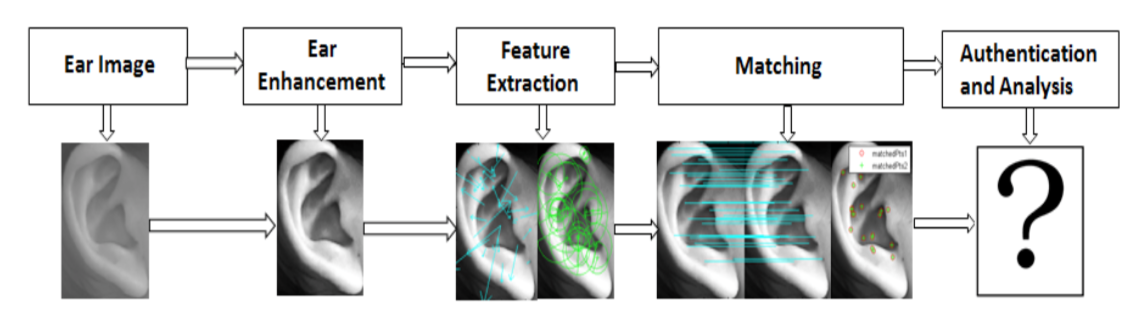
\includegraphics[width=\textwidth]{Figures/Figure1}
	\caption{The pipeline of the proposed Ear Recognition System}
	\label{fig:Figure1}
\end{figure}
Extensive experiments have been carried out on two different sets of databases to evaluate their performance with respect to various rotations and scales. One of the most important feature of ear images is its easiness in acquisition, however, the acquired images may be in different scales, rotations, and illumination. The scale and rotation invariant property of the SIFT and SURF algorithms makes them perfect for ear authentication under various circumstances.

 A new concept in the field of machine learning and computer vision has come up which has surpassed the traditional object recognition methods. This new approach is called deep learning. Deep Learning is a branch of Machine Learning which has multiple levels of representations and abstractions. It is basically a rebranding of the term Artificial Neural Networks. Deep Learning algorithms have already been applied in Apple's Siri, Google's Streetview etc. 
 
 The reason behind the rise of ear biometrics is that the structure of the ear is not only unique but also permanent. Since the acquisition of ear images does not require a person's co-operation, due to these advantages the interest in ear recognition research has grown significantly in the past few years. One of the most important challenges in ear biometrics is occlusion and pose variation, in contrast to the face, the ear is sometimes partially occluded by hair, ear-rings, headphones. Robustness against occlusions have been addressed in previous publications \cite{pflug2012ear}. But no studies have been covered on the effect of certain types of occlusion like hair or earrings. 
 
 Pose variations has also been another challenge in this domain where the subject's ear is never straight and is moving all the time when the images are captured from different angles. Thus scalability and pose remains a concern. In this project, details on pose variations and scales have been provided and analysis has also been done to see how it affects the performance of the system.
 
 The symmetry of the right and left ear has not been understood yet.The studies of Iannarelli indicates that some characteristics of the outer ear can be inherited and another factor is ageing. These assumptions does not have a proof since ear recognition is still a relatively new field of research. Lighting condtitions, pose variations till remain a great challenge to the performance of the biometric systems. Though good databases are available, it is still difficult to get better performances as most of the databases follow a specific standard and they are taken under the same light and pose variations.
 
 

The rest  is organized as follows. Some background and related research are discussed in Section 2; the proposed method is presented in details in Section 3; some experimental results and analysis are given in Section 4; and the paper is concluded in Section 5.
